\newcommand{\drawtruss}[2][1]{%
\begin{center}
\begin{tikzpicture}[scale=#1, every node/.style={scale=#1}]
\draw (0,0) node[left,magenta]{C} -- 
      (1,1.71) node[left,magenta]{A} -- 
      (2,0) node[above,magenta]{D} -- cycle;
\draw (2,0) -- 
      (3,1.71) node[right,magenta]{B} -- 
      (1,1.71) -- cycle;
\draw (3,1.71) -- (4,0) node[right,magenta]{E} -- (2,0) -- cycle;
\draw[blue] (0,0) -- (0.25,-0.425) -- (-0.25,-0.425) -- cycle;
\draw[blue] (4,0) -- (4.25,-0.425) -- (3.75,-0.425) -- cycle;
\draw[thick,red,->] (2,0) -- (2,-0.75);
#2
\end{tikzpicture}
\end{center}
}
\newcommand{\trussNormalForces}{%
\draw [thick, blue,->] (0,0) -- (0.5,0.5);
\draw [thick, blue,->] (4,0) -- (3.5,0.5);
}
\newcommand{\trussCompletion}{%
\trussNormalForces
\draw [thick, magenta,<->] (0.4,0.684) -- (0.6,1.026);
\draw [thick, magenta,<->] (3.4,1.026) -- (3.6,0.684);
\draw [thick, magenta,<->] (1.8,1.71) -- (2.2,1.71);
\draw [thick, magenta,->] (1.6,0.684) -- (1.5,0.855);
\draw [thick, magenta,<-] (1.5,0.855) -- (1.4,1.026);
\draw [thick, magenta,->] (2.4,0.684) -- (2.5,0.855);
\draw [thick, magenta,<-] (2.5,0.855) -- (2.6,1.026);
}
\newcommand{\trussCForces}{%
\draw [thick, blue,->] (0,0) -- (0.5,0.5);
\draw [thick, magenta,->] (0,0) -- (0.4,0.684);
\draw [thick, magenta,->] (0,0) -- (0.5,0);
}
\newcommand{\trussStrutVariables}{%
\node[above] at (2,1.71) {\(x_1\)};
\node[left] at (0.5,0.866) {\(x_2\)};
\node[left] at (1.5,0.866) {\(x_3\)};
\node[right] at (2.5,0.866) {\(x_4\)};
\node[right] at (3.5,0.866) {\(x_5\)};
\node[below] at (1,0) {\(x_6\)};
\node[below] at (3,0) {\(x_7\)};
}

\begin{applicationActivities}

\begin{example}
In engineering, a \term{truss} is a structure designed from several beams
of material called \term{struts}, assembled to behave as a single object.

\begin{center}
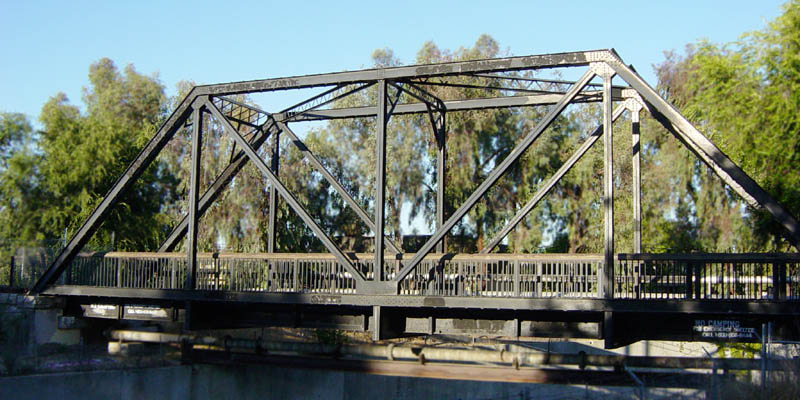
\includegraphics[width=0.8\linewidth]{media/truss.jpg}
\end{center}
\end{example}

\begin{activity}{5}
Consider the representation of a simple truss pictured below.
All of the seven struts are of equal length, affixed to two anchor points
applying a normal force to nodes \(C\) and \(E\), and
with a \(10000 N\) load applied to the node given by \(D\).

\drawtruss{}

Which of the following must hold for the truss to be stable?
\begin{enumerate}[a)]
\item All of the struts will experience compression.
\item All of the struts will experience tension.
\item Some of the struts will be compressed, but others will be tensioned.
\end{enumerate}
\end{activity}

\begin{observation}
Since the forces must balance at each node for the truss to be stable,
some of the struts will be compressed, while others will be tensioned. 

\drawtruss{\trussCompletion}

By finding vector equations that must hold at each node, we may
determine many of the forces at play.
\end{observation}

\begin{remark}
For example, at the bottom left node there are 3 forces acting.

\drawtruss{\trussCForces}

Let \(\vec F_{CA}\) be the force on \(C\) given by the compression/tension
of the strut \(CA\), let \(\vec F_{CD}\) be defined similarly, and let
\(\vec N_C\) be the normal force of the anchor point on \(C\).

\vspace{1em}

For the truss to be stable, we must have
\[
\vec F_{CA}+\vec F_{CD}+\vec N_C=\vec 0
.\]
\end{remark}

\begin{activity}{10}
Using the conventions of the previous slide, and where \(\vec L\)
represents the load vector on node \(D\), find four more vector equations
that must be satisfied for each of the other four nodes of the truss.

\drawtruss

\[
A: \unknown
\]
\[
B: \unknown
\]
\[
C: \vec F_{CA}+\vec F_{CD}+\vec N_C=\vec 0
\]
\[D:\unknown\]
\[E:\unknown\]
\end{activity}

\begin{remark}
The five vector equations may be written as follows.

\drawtruss

\[
A: \vec F_{AC}+\vec F_{AD}+\vec F_{AB}=\vec 0
\]
\[
B: \vec F_{BC}+\vec F_{BD}+\vec F_{BE}=\vec 0
\]
\[
C: \vec F_{CA}+\vec F_{CD}+\vec N_C=\vec 0
\]
\[
D: \vec F_{DC}+\vec F_{DA}+\vec F_{DB} +\vec F_{DE}+\vec L=\vec 0
\]
\[
E: \vec F_{EB}+\vec F_{ED}+\vec N_E=\vec 0
\]
\end{remark}

%\begin{activity}{5}
%An augmented matrix representing these five equations would have how many rows?
%\[
%A: \vec F_{AC}+\vec F_{AD}+\vec F_{AB}=\vec 0
%\]
%\[
%B: \vec F_{BC}+\vec F_{BD}+\vec F_{BE}=\vec 0
%\]
%\[
%C: \vec F_{CA}+\vec F_{CD}+\vec N_C=\vec 0
%\]
%\[
%D: \vec F_{DC}+\vec F_{DA}+\vec F_{DB} +\vec F_{DE}+\vec L=\vec 0
%\]
%\[
%E: \vec F_{EB}+\vec F_{ED}+\vec N_E=\vec 0
%\]
%\begin{enumerate}[a)]
%\item 5
%\item 10
%\item 25
%\end{enumerate}
%\end{activity}

\begin{observation}
\drawtruss{}

Each vector may be treated as an \(\IR^2\) vector by
decomposing its magnitude into vertical and horizontal components.
Note that \(\vec F_{CA}\) must have the same magnitude (and opposite
direction) as \(\vec F_{AC}\).

\[
  \vec{F}_{CA}
    = 
  x\begin{bmatrix} \cos(60^\circ) \\ \sin(60^\circ) \end{bmatrix}
    =
  x\begin{bmatrix} 1/2 \\ \sqrt{3}/2\end{bmatrix}
\]

\[
  \vec{F}_{AC}
    = 
  x\begin{bmatrix} \cos(-120^\circ) \\ \sin(-120^\circ) \end{bmatrix}
    =
  x\begin{bmatrix} -1/2 \\ -\sqrt{3}/2\end{bmatrix}
\]
\end{observation}

\begin{activity}{5}
To write a linear system that models the truss under consideration,
how many variables will be required?

\drawtruss{}

\begin{enumerate}[a)]
\item \(7\): \(5\) from the nodes, \(2\) from the anchors
\item \(10\): \(7\) from the struts, \(2\) from the anchors, \(1\) from the load
\item \(11\): \(7\) from the struts, \(4\) from the anchors
\item \(13\): \(5\) from the nodes, \(7\) from the struts, \(1\) from the load
\end{enumerate}
\end{activity}

\begin{observation}
Since the angles for each strut are known,
one variable may be used to represent each.

\drawtruss{\trussStrutVariables}

For example:

\[
\vec F_{AB}=-\vec F_{BA}=x_1\begin{bmatrix}\cos(0)\\\sin(0)\end{bmatrix}
=x_1\begin{bmatrix}1\\0\end{bmatrix}
\]
\[
\vec F_{BE}=-\vec F_{EB}=x_5\begin{bmatrix}\cos(-60^\circ)\\\sin(-60^\circ)\end{bmatrix}
=x_5\begin{bmatrix}1/2\\-\sqrt{3}/2\end{bmatrix}
\]


\end{observation}

\begin{observation}
Since the angle of the normal forces for each anchor point are unknown,
two variables may be used to represent each.

\drawtruss{\trussNormalForces}

\[
\vec N_C=\begin{bmatrix}y_1\\y_2\end{bmatrix}
\hspace{3em}
\vec N_D=\begin{bmatrix}z_1\\z_2\end{bmatrix}
\]

The load vector is constant.

\[
\vec L = \begin{bmatrix}0\\-10000\end{bmatrix}
\]

\end{observation}

\begin{remark}
Each of the five vector
equations found previously represent two linear equations:
one for the horizontal component and one for the vertical.

\drawtruss{\trussStrutVariables}

\[
C: \vec F_{CA}+\vec F_{CD}+\vec N_C=\vec 0
\]
\[
\Leftrightarrow
x_2\begin{bmatrix}\cos(60^\circ)\\\sin(60^\circ)\end{bmatrix}+
x_6\begin{bmatrix}\cos(0^\circ)\\\sin(0^\circ)\end{bmatrix}+
\begin{bmatrix}y_1\\y_2\end{bmatrix}=\begin{bmatrix}0\\0\end{bmatrix}
\]
Using the approximation \(\sqrt{3}/2\approx 0.866\), we have
\[
\Leftrightarrow
x_2\begin{bmatrix}0.5\\0.866\end{bmatrix}+
x_6\begin{bmatrix}1\\0\end{bmatrix}+
y_1\begin{bmatrix}1\\0\end{bmatrix}+
y_2\begin{bmatrix}0\\1\end{bmatrix}=
\begin{bmatrix}0\\0\end{bmatrix}
\]
\end{remark}

\begin{activity}{10}
Expand the vector equation given below using sine and cosine of appropriate angles,
then compute each component (approximating \(\sqrt{3}/2\approx 0.866\)).

\drawtruss{\trussStrutVariables}

\[
D:\vec F_{DA}+\vec F_{DB}+\vec F_{DC}+\vec F_{DE}=-\vec L
\]
\[
\Leftrightarrow
x_3\begin{bmatrix}\cos(\unknown)\\\sin(\unknown)\end{bmatrix}+
x_4\begin{bmatrix}\cos(\unknown)\\\sin(\unknown)\end{bmatrix}+
x_6\begin{bmatrix}\cos(\unknown)\\\sin(\unknown)\end{bmatrix}+
x_7\begin{bmatrix}\cos(\unknown)\\\sin(\unknown)\end{bmatrix}=
\begin{bmatrix}\unknown\\\unknown\end{bmatrix}
\]
\[
\Leftrightarrow
x_3\begin{bmatrix}\unknown\\\unknown\end{bmatrix}+
x_4\begin{bmatrix}\unknown\\\unknown\end{bmatrix}+
x_6\begin{bmatrix}\unknown\\\unknown\end{bmatrix}+
x_7\begin{bmatrix}\unknown\\\unknown\end{bmatrix}=
\begin{bmatrix}\unknown\\\unknown\end{bmatrix}
\]

\end{activity}

\begin{observation}
The full augmented matrix given by the ten equations in this linear system
is given below, where the elevent columns correspond to \(x_1,\dots,x_7,y_1,y_2,z_1,z_2\),
and the ten rows correspond to the horizontal and vertical components of the
forces acting at \(A,\dots,E\).

%\drawtruss[0.7]{\trussStrutVariables}

\[
\begin{bmatrix}[ccccccccccc|c]
1&-0.5&0.5&0&0&0&0&0&0&0&0&0\\
0&-0.866&-0.866&0&0&0&0&0&0&0&0&0\\
-1&0&0&-0.5&0.5&0&0&0&0&0&0&0\\
0&0&0&-0.866&-0.866&0&0&0&0&0&0&0\\
0&0.5&0&0&0&1&0&1&0&0&0&0\\
0&0.866&0&0&0&0&0&0&1&0&0&0\\
0&0&-0.5&0.5&0&-1&1&0&0&0&0&0\\
0&0&0.866&0.866&0&0&0&0&0&0&0&10000\\
0&0&0&0&-0.5&0&-1&0&0&1&0&0\\
0&0&0&0&0.866&0&0&0&0&0&1&0\\
\end{bmatrix}
\]
\end{observation}

\begin{observation}
This matrix row-reduces to the following.

%\drawtruss[0.7]{\trussStrutVariables}

\[\sim
\begin{bmatrix}[ccccccccccc|c]
1&0&0&0&0&0&0&0&0&0&0&-5773.7\\
0&1&0&0&0&0&0&0&0&0&0&-5773.7\\
0&0&1&0&0&0&0&0&0&0&0&5773.7\\
0&0&0&1&0&0&0&0&0&0&0&5773.7\\
0&0&0&0&1&0&0&0&0&0&0&-5773.7\\
0&0&0&0&0&1&0&0&0&-1&0&2886.8\\
0&0&0&0&0&0&1&0&0&-1&0&2886.8\\
0&0&0&0&0&0&0&1&0&1&0&0\\
0&0&0&0&0&0&0&0&1&0&0&5000\\
0&0&0&0&0&0&0&0&0&0&1&5000\\
\end{bmatrix}
\]
\end{observation}
\begin{observation}
\drawtruss{\trussCompletion}

Thus we know the truss must satisfy the following conditions.
\begin{align*}
x_1=x_2=x_5&=-5882.4 \\
x_3=x_4&=5882.4\\
x_6=x_7&=2886.8+z_1\\
y_1&=-z_1\\
y_2=z_2&=5000 \\
\end{align*}
In particular, the negative \(x_1,x_2,x_5\) represent tension (forces pointing into the nodes),
and the postive \(x_3,x_4\) represent compression (forces pointing out of the nodes).
The vertical normal forces \(y_2+z_2\) counteract the \(10000\) load.

\end{observation}



\end{applicationActivities}
